\documentclass[../main.tex]{subfiles}

\begin{document}
    
\subsubsection*{Methodology}
    Next, the dependance on the lasing power of the resonator length $L$ will be investigated. Concretely, the loss controlled by $L$ will be quantified. For this, the setup in figure \ref{fig:4-Aufbau} is used.
    
    \begin{figure}[H]
        \centering 
        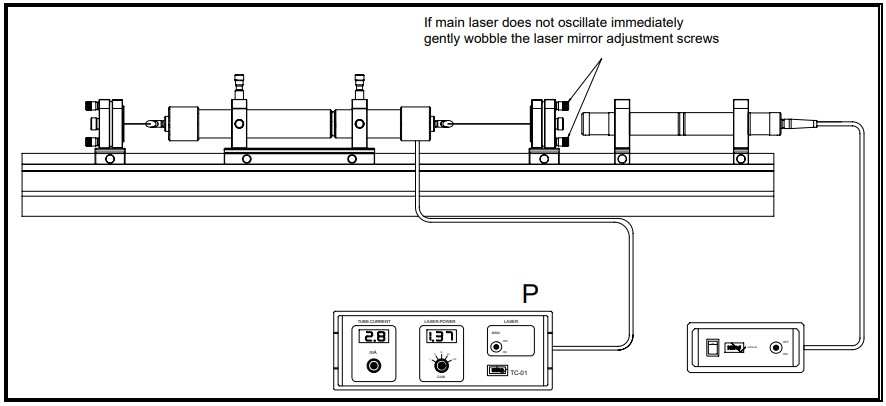
\includegraphics[width = 11cm]{Bilddateien/4/4-Aufbau.jpg}
        \caption{Experimental setup for optical stability of the laser. The components displayed are from left to right: left laser mirror holder (A), main laser tube (B), right laser mirror holder (D), pilot laser (E). For the measurment of the laser spectrum a spectrometer can be placed left to the left laser mirror holder (A) \cite[p.22]{doc:HeNeStudentManual}.}
        \label{fig:4-Aufbau}
    \end{figure}

    \noindent The resonator length is then varied from $L = \SI{60.5}{\cm}$ to $L = \SI{71}{\cm}$ and for each configuration, the lasing power is measured. Slight adjustments to the resonator mirrror holders (A), (D) and the main laser tube (B) have to be made for each length $L$ to achieve optimal lasing for the occuring light modes.

\subsubsection*{Data analysis}
    Figure \ref{fig:4-Laserleistung-Resonatorlaenge} shows the laser output power plottet against the length of the resonator (measured from the left laser holder to the right laser holder). A general decline of laser power for larger resonator lengths can be seem, which saturates at roughly \SI{0.5(10)}{\mW} (mean value of the last three data points). This can be explained by the fact that for a larger ocscillation length $L$ of the laser modes, the number of light configurations (distance of ray from optical axis, light divergence) that lead to modes escaping the resonator grows: e.g. even if a light ray has a small angle of divergence $\alpha$ after being reflected from the left resonator, the distance $x$ from the optical axis when reaching the right resonator, $x = \sin(\alpha)\cdot L$ may be greater than the resonator width, provided $L$ is large enough. For a plane parallel mirror and a curved one of curvature radius $R$, the maximum limit $L_{th}$ where stable light modes in the resonator are still possible is given by \cite[p.15]{doc:HeNeStudentManual} 
    \[
        0 \le 1 - \frac{R}{L_{th}} \le 1 \implies L_{th}.    
    \]
    A linear fit of the shape $P(L) = \alpha\cdot (L - L_{th})$ was chosen as a rough estimate for the threshold length $L_{th}$ for lasing. The data points more closely resemble a curve with first negative and then positive curvature, but on average a linear fit seems sufficient.

    \begin{figure}[H]
        \centering
        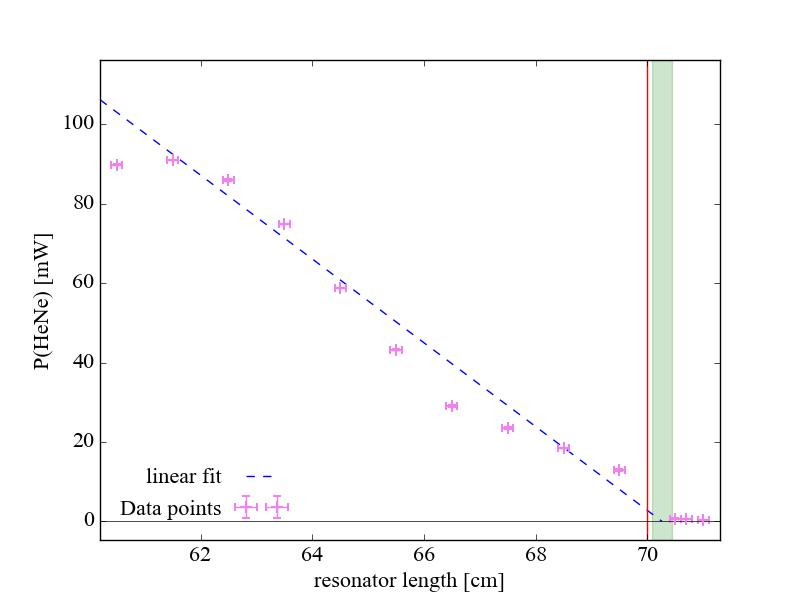
\includegraphics[width = 11cm]{Bilddateien/4/4-Laserleistung-Resonatorlaenge.jpg}
        \caption{Dependance of laser power from resonator length. The red vertical line represents the theoretical maximum resonator length $\color{red}{\SI{70}{\cm}}$, where lasing still occours. Its experimental counterpart $\color{ForestGreen}{L_{th} = \SI{70.26(18)}{\cm}}$  is colored green.}
        \label{fig:4-Laserleistung-Resonatorlaenge}
    \end{figure}

    \noindent Even though the theoretical and experimental values for the threshold length are not comptatible according to their uncertainties, they are less than $\SI{3}{\mm}$ to each other. The remaining power of \SI{0.5(10)}{\mW} measured for $L > L_{th}$ is most likely due to background static.

\end{document}